The research outpost \textit{Polaris Deep} orbits a dying star, and its only protection from the heat is a coolant network laid out on a grid of $n \times m$ tiles. Each tile is either empty or holds a junction. A junction has openings in two, three, or four of the four cardinal directions --- up, right, down, left. A junction with exactly one opening is physically impossible: the pressure would burst it instantly.

Two junctions in orthogonally adjacent tiles are \emph{connected} if and only if both have openings facing each other. A \emph{loop} is a route that starts at some junction, moves along connections, and returns to the starting junction without using any connection twice.

The chief engineer measures the network's resilience by the number of \emph{independent loops}$^{\dagger}$ it contains.

Each tile is described by a single integer $g_{i,j}$: $0$ for an empty tile, and otherwise the sum of $1$ for an opening facing up, $2$ for right, $4$ for down, and $8$ for left. For instance, a junction whose openings face up and right is written as $g_{i,j} = 1 + 2 = 3$:

\begin{center}
  \def \htmlPixelsInCm {45}
  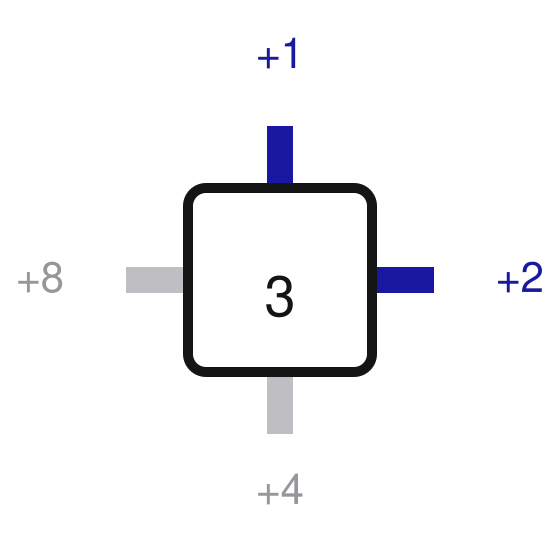
\includegraphics[width=3cm]{pipe-bits.svg}
\end{center}

Openings facing outside the grid connect to nothing.

During a micrometeorite storm the junctions are destroyed one by one. Telemetry predicts the whole sequence of $q$ impacts in advance: every impact hits a tile containing a working junction, and no tile is hit twice.

After each impact, report the number of independent loops remaining in the network.

{\small $^{\dagger}$ Formally, the \emph{number of independent loops} of the network is the largest $t$ for which one can choose a sequence of loops $L_1, L_2, \ldots, L_t$ such that every loop $L_i$ passes through at least one connection that none of the earlier loops $L_1, L_2, \ldots, L_{i-1}$ pass through.}
